\subsection{UC4 - Visualizzazione libreria}
\begin{figure}[H]
  \centering
  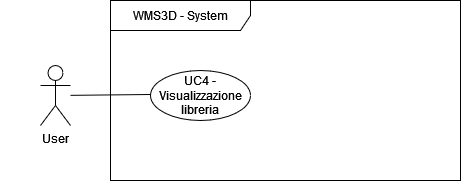
\includegraphics[width=0.8\textwidth]{UC_diagrams_1-10/UC4_sys.drawio.png}
   \caption{Diagramma UML UC4 - Visualizzazione libreria}
\end{figure}
\begin{figure}[H]
  \centering
  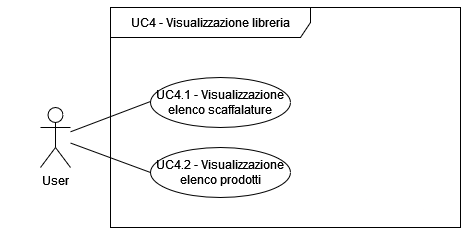
\includegraphics[width=0.8\textwidth]{UC_diagrams_1-10/UC4.drawio.png}
   \caption{Diagramma UML in dettaglio UC4 - Visualizzazione libreria}
\end{figure}
\begin{itemize}
    \item \textbf{Attori:} User.
    \item \textbf{Pre-condizione:}  L'utente ha creato un magazzino [UC1].
    \item \textbf{Post-condizione:} L'utente visualizza in una parte dell'applicazione uno spazio riservato alle informazioni testuali riguardanti gli elementi (scaffalature e prodotti) interni al magazzino (i.e. la libreria\textsuperscript{G}).
    \item \textbf{Scenario Principale:}  L'utente può visualizzare in libreria, un elenco delle scaffalature [UC4.1] e uno dei prodotti [UC4.2] (con relativi dati), sempre se presenti all'interno del magazzino. Se non vi dovessero essere nessuno di questi elementi, lo spazio verrà visualizzato vuoto.
    \item \textbf{Generalizzazioni:} -
    \item \textbf{Estensioni:} -
\end{itemize}


\subsubsection{UC4.1 - Visualizzazione elenco scaffalature}
\begin{figure}[H]
  \centering
  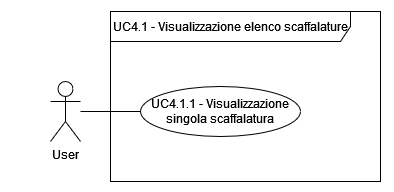
\includegraphics[width=0.8\textwidth]{UC_diagrams_1-10/UC4.1.drawio.png}
   \caption{Diagramma UML UC4.1 - Visualizzazione elenco scaffalature}
\end{figure}
\begin{itemize}
    \item \textbf{Attori:} User.
    \item \textbf{Pre-condizione:}  L'utente ha creato un magazzino [UC1] e ne sta guardando la libreria.
    \item \textbf{Post-condizione:} L'utente può vedere i dati relativi a tutte le scaffalature presenti nel magazzino.
    \item \textbf{Scenario Principale:} L'utente può visualizzare in libreria ogni singola scaffalatura [UC4.1.1] (con relativi dati), sempre se presenti all'interno del magazzino. Se non vi dovesse essere nessuna scaffalatura, l'elenco sarà nullo.
    \item \textbf{Generalizzazioni:} -
    \item \textbf{Estensioni:} -
\end{itemize}


\paragraph{UC4.1.1 - Visualizzazione singola scaffalatura}
\begin{figure}[H]
  \centering
  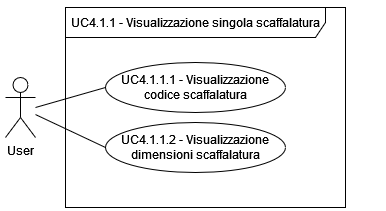
\includegraphics[width=0.7\textwidth]{UC_diagrams_1-10/UC4.1.1.drawio.png}
   \caption{Diagramma UML UC4.1.1 - Visualizzazione singola scaffalatura}
\end{figure}
\begin{itemize}
    \item \textbf{Attori:} User.
    \item \textbf{Pre-condizione:} L'utente ha creato un magazzino [UC1] e sta guardando all'elenco delle scaffalature interno alla libreria. Almeno una scaffalatura deve essere creata [UC6] e posizionata [UC7].
    \item \textbf{Post-condizione:} L'utente può vedere i dati relativi ad una singola scaffalatura.
    \item \textbf{Scenario Principale:} L'utente può visualizzare il codice identificativo [UC4.1.1.1], la capacità in bin [UC4.1.1.2] e le dimensioni del bin [UC4.1.1.3] per ogni singola scaffalatura presente nella libreria.
    \item \textbf{Generalizzazioni:} -
    \item \textbf{Estensioni:} -
\end{itemize}


\paragraph{UC4.1.1.1 - Visualizzazione codice scaffalatura}
\begin{itemize}
    \item \textbf{Attori:} User.
    \item \textbf{Pre-condizione:} L'utente ha creato un magazzino [UC1] e sta guardando ad una singola scaffalatura all'interno della libreria. Pertanto, almeno una scaffalatura deve essere creata [UC6] e posizionata [UC7].
    \item \textbf{Post-condizione:} L'utente può vedere il codice relativo alla singola scaffalatura.
    \item \textbf{Scenario Principale:} L'utente può visualizzare il codice identificativo per ogni singola scaffalatura presente nella libreria.
    \item \textbf{Generalizzazioni:} -
    \item \textbf{Estensioni:} -
\end{itemize}


\paragraph{UC4.1.1.2 - Visualizzazione dimensioni scaffalatura}
\begin{figure}[H]
  \centering
  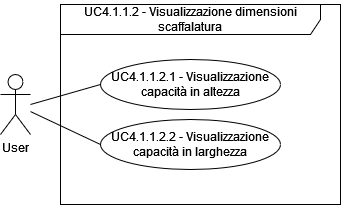
\includegraphics[width=0.8\textwidth]{UC_diagrams_1-10/UC4.1.1.2.drawio.png}
   \caption{Diagramma UML UC4.1.1.2 - Visualizzazione dimensioni scaffalatura}
\end{figure}
\begin{itemize}
    \item \textbf{Attori:} User.
    \item \textbf{Pre-condizione:} L'utente ha creato un magazzino [UC1] e sta guardando ad una singola scaffalatura all'interno della libreria. Pertanto, almeno una scaffalatura deve essere creata [UC6] e posizionata [UC7].
    \item \textbf{Post-condizione:} L'utente può vedere le dimensioni relative alla singola scaffalatura.
    \item \textbf{Scenario Principale:} L'utente può visualizzare le dimensioni, quindi capacità in altezza [UC4.1.1.2.1] e capacità in larghezza [UC4.1.1.2.2], per ogni singola scaffalatura presente nella libreria.
    \item \textbf{Generalizzazioni:} -
    \item \textbf{Estensioni:} -
\end{itemize}


\paragraph{UC4.1.1.2.1 - Visualizzazione capacità in altezza}
\begin{itemize}
    \item \textbf{Attori:} User.
    \item \textbf{Pre-condizione:} L'utente ha creato un magazzino [UC1] e sta guardando ad una singola scaffalatura all'interno della libreria. Pertanto, almeno una scaffalatura deve essere creata [UC6] e posizionata [UC7].
    \item \textbf{Post-condizione:} L'utente può vedere la capacità in altezza relativa alla singola scaffalatura.
    \item \textbf{Scenario Principale:} L'utente può visualizzare la capacità (i.e. numero di bin) in altezza per ogni singola scaffalatura presente nella libreria.
    \item \textbf{Generalizzazioni:} -
    \item \textbf{Estensioni:} -
\end{itemize}


\paragraph{UC4.1.1.2.2 - Visualizzazione capacità in larghezza}
\begin{itemize}
    \item \textbf{Attori:} User.
    \item \textbf{Pre-condizione:} L'utente ha creato un magazzino [UC1] e sta guardando ad una singola scaffalatura all'interno della libreria. Pertanto, almeno una scaffalatura deve essere creata [UC6] e posizionata [UC7].
    \item \textbf{Post-condizione:} L'utente può vedere la capacità in larghezza relativa alla singola scaffalatura.
    \item \textbf{Scenario Principale:}  L'utente può visualizzare la capacità (i.e. numero di bin) in larghezza per ogni singola scaffalatura presente nella libreria.
    \item \textbf{Generalizzazioni:} -
    \item \textbf{Estensioni:} -
\end{itemize}


\paragraph{UC4.1.1.3 - Visualizzazione dimensioni singolo bin}
\begin{figure}[H]
  \centering
  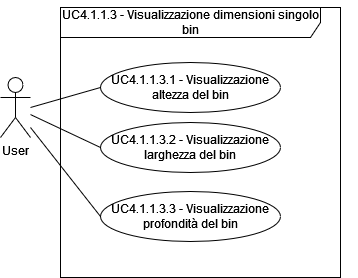
\includegraphics[width=0.8\textwidth]{UC_diagrams_1-10/UC4.1.1.3.drawio.png}
   \caption{Diagramma UML UC4.1.1.3 - Visualizzazione dimensioni singolo bin}
\end{figure}
\begin{itemize}
    \item \textbf{Attori:} User.
    \item \textbf{Pre-condizione:} L'utente ha creato un magazzino [UC1] e sta guardando ad una singola scaffalatura all'interno della libreria. Pertanto, almeno una scaffalatura deve essere creata [UC6] e posizionata [UC7].
    \item \textbf{Post-condizione:} L'utente può vedere le dimensioni relative al singolo bin interno alla scaffalatura.
    \item \textbf{Scenario Principale:} L'utente può visualizzare le dimensioni, quindi altezza [UC4.1.1.3.1], larghezza [UC4.1.1.3.2] e profondità [UC4.1.1.3.3], dei bin di cui la scaffalatura è composta.
    \item \textbf{Generalizzazioni:} -
    \item \textbf{Estensioni:} -
\end{itemize}

\paragraph{UC4.1.1.3.1 - Visualizzazione altezza del bin}
\begin{itemize}
    \item \textbf{Attori:} User.
    \item \textbf{Pre-condizione:} L'utente ha creato un magazzino [UC1] e sta guardando ad una singola scaffalatura all'interno della libreria. Pertanto, almeno una scaffalatura deve essere creata [UC6] e posizionata [UC7].
    \item \textbf{Post-condizione:} L'utente può vedere la dimensione in altezza relativa al singolo bin della scaffalatura.
    \item \textbf{Scenario Principale:} L'utente può visualizzare l'altezza del bin per ogni scaffalatura presente nella libreria.
    \item \textbf{Generalizzazioni:} -
    \item \textbf{Estensioni:} -
\end{itemize}


\paragraph{UC4.1.1.3.2 - Visualizzazione larghezza del bin}
\begin{itemize}
    \item \textbf{Attori:} User.
    \item \textbf{Pre-condizione:} L'utente ha creato un magazzino [UC1] e sta guardando ad una singola scaffalatura all'interno della libreria. Pertanto, almeno una scaffalatura deve essere creata [UC6] e posizionata [UC7].
    \item \textbf{Post-condizione:} L'utente può vedere la dimensione in larghezza relativa al singolo bin della scaffalatura.
    \item \textbf{Scenario Principale:}  L'utente può visualizzare la larghezza del bin per ogni scaffalatura presente nella libreria.
    \item \textbf{Generalizzazioni:} -
    \item \textbf{Estensioni:} -
\end{itemize}

\paragraph{UC4.1.1.3.3 - Visualizzazione profondità del bin}
\begin{itemize}
    \item \textbf{Attori:} User.
    \item \textbf{Pre-condizione:} L'utente ha creato un magazzino [UC1] e sta guardando ad una singola scaffalatura all'interno della libreria. Pertanto, almeno una scaffalatura deve essere creata [UC6] e posizionata [UC7].
    \item \textbf{Post-condizione:} L'utente può vedere la dimensione in profondità relativa al singolo bin della scaffalatura.
    \item \textbf{Scenario Principale:} L'utente può visualizzare la profondità del bin per ogni scaffalatura presente nella libreria.
    \item \textbf{Generalizzazioni:} -
    \item \textbf{Estensioni:} -
\end{itemize}


\subsubsection{UC4.2 - Visualizzazione elenco prodotti}
\begin{figure}[H]
  \centering
  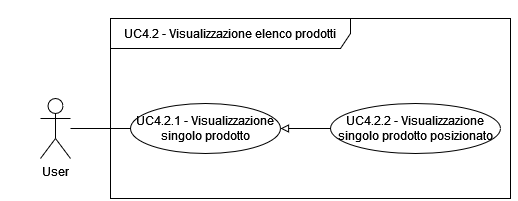
\includegraphics[width=0.8\textwidth]{UC_diagrams_1-10/UC4.2.drawio.png}
   \caption{Diagramma UML UC4.2 - Visualizzazione elenco prodotti}
\end{figure}
\begin{itemize}
    \item \textbf{Attori:} User.
    \item \textbf{Pre-condizione:}  L'utente ha creato un magazzino [UC1] e ne sta guardando la libreria.
    \item \textbf{Post-condizione:} L'utente può vedere i dati relativi a tutti i prodotti presenti nel magazzino.
    \item \textbf{Scenario Principale:} L'utente può visualizzare in libreria ogni singolo prodotto [UC4.2.1] (con relativi dati), posizionato o meno. Se non vi dovesse essere nessun prodotto, l'elenco sarà nullo.
    \item \textbf{Generalizzazioni:} -
    \item \textbf{Estensioni:} -
\end{itemize}


\paragraph{UC4.2.1 - Visualizzazione singolo prodotto}
\begin{figure}[H]
  \centering
  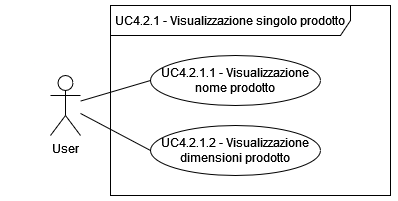
\includegraphics[width=0.8\textwidth]{UC_diagrams_1-10/UC4.2.1.drawio.png}
   \caption{Diagramma UML UC4.2.1 - Visualizzazione singolo prodotto}
\end{figure}
\begin{itemize} 
    \item \textbf{Attori:} User.
    \item \textbf{Pre-condizione:}  L'utente ha creato un magazzino [UC1] e sta guardando all'elenco dei prodotti interno alla libreria. Almeno un prodotto deve essere stato creato [UC13].
    \item \textbf{Post-condizione:} L'utente può vedere i dati relativi ad un singolo prodotto.
    \item \textbf{Scenario Principale:} L'utente può visualizzare il nome [UC4.2.1.1] per ogni singolo prodotto presente nella libreria. 
    \item \textbf{Generalizzazioni:} È presente una generalizzazione:
    \begin{itemize}
        \item UC4.2.2 - Visualizzazione singolo prodotto posizionato
    \end{itemize}
    \item \textbf{Estensioni:} -
\end{itemize}


\paragraph{UC4.2.1.1 - Visualizzazione nome prodotto}
\begin{itemize} 
    \item \textbf{Attori:} User.
    \item \textbf{Pre-condizione:}  L'utente ha creato un magazzino [UC1] e sta guardando ad un singolo prodotto all'interno della libreria. Almeno un prodotto deve essere stato creato [UC13].
    \item \textbf{Post-condizione:} L'utente può vedere il nome del prodotto.
    \item \textbf{Scenario Principale:} L'utente può visualizzare il nome per ogni singolo prodotto presente nella libreria. 
    \item \textbf{Generalizzazioni:} -
    \item \textbf{Estensioni:} -
\end{itemize}


\paragraph{UC4.2.2 - Visualizzazione singolo prodotto posizionato}
\begin{figure}[H]
  \centering
  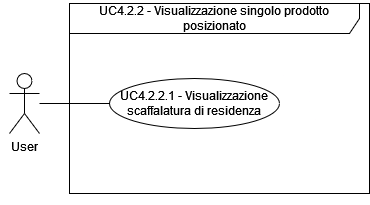
\includegraphics[width=0.8\textwidth]{UC_diagrams_1-10/UC4.2.2.drawio.png}
   \caption{Diagramma UML UC4.2.2 - Visualizzazione singolo prodotto posizionato}
\end{figure}
\begin{itemize}
    \item \textbf{Attori:} User.
    \item \textbf{Pre-condizione:}  L'utente ha creato un magazzino [UC1] e sta guardando all'elenco dei prodotti interno alla libreria. Almeno un prodotto deve essere stato creato [UC13] e posizionato [UC14].
    \item \textbf{Post-condizione:}  L'utente può vedere i dati relativi ad un singolo prodotto.
    \item \textbf{Scenario Principale:}  L'utente può visualizzare il nome [UC4.2.1.1] per ogni singolo prodotto ed, essendo posizionato, anche la scaffalatura in cui il prodotto risiede [4.2.2.1]. 
    \item \textbf{Generalizzazioni:} -
    \item \textbf{Estensioni:} -
\end{itemize}


\paragraph{UC4.2.2.1 - Visualizzazione scaffalatura di residenza}
\begin{itemize} 
    \item \textbf{Attori:} User.
    \item \textbf{Pre-condizione:}  L'utente ha creato un magazzino [UC1] e sta guardando ad un singolo prodotto all'interno della libreria. Almeno un prodotto deve essere stato creato [UC13] e posizionato [UC14].
    \item \textbf{Post-condizione:} L'utente può vedere la scaffalatura di residenza di un prodotto posizionato.
    \item \textbf{Scenario Principale:} L'utente può visualizzare la posizione, ovvero il codice della scaffalatura in cui il prodotto si trova, per ogni singolo prodotto posizionato presente nella libreria. 
    \item \textbf{Generalizzazioni:} -
    \item \textbf{Estensioni:} -
\end{itemize}